\setchapterpreamble[u]{\margintoc}
\chapter{李群(Lie Group)与李代数(Lie Algebra)}
\labch{intro}


\section*{章节导论:对称性与对称性破缺}
仍在画饼,可以参考这篇知乎文章,写的很不错:\href{https://zhuanlan.zhihu.com/p/338221764}{知乎专栏}




\section{李群(Lie Group)初步}
\subsection{群与李群(Lie Group)}
我们或许听说过一个说法:``物理学的关键是对称和守恒",而诺特定理给出了对称性与守恒性的联系,例如,时间平移不变性意味着能量守恒;空间平移不变性意味着动量守恒;转动不变性意味着角动量守恒;电势和向量势的规范不变性得出电荷的守恒等.而描述对称性的语言就是群论.


我们可以认为群是一类拥有特殊结构的集合,即满足如下关系的集合\sidenote[][]{当然,这里会忽略对于主线无用的那些群论内容,所以如果和数学系的抽象代数对比,你甚至可能会感觉到学的不是同一个东西}:
\marginnote[]{这一章虽然名字比较吓人,但并没有太过深入讲解李群与李代数,主要为了帮助物理系学生来快速对这一门学科建立印象.当然,我们不能保证在后续的不断更新中是否会改变这一点,在最初的版本中,这一章被置于第三章,也就是初量的后续部分,以及这一章的进度只会跟进后续章节的需要,也就是说这一章的全部已完成内容足以支撑起后续章节的学习.}
\begin{definition}[群的定义]
    设$G$是一个集合,若满足下面4个条件,则称$G$为一个群(Group)
    \begin{enumerate}
        \item $G$中存在一种运算规则,对$G$中的任意两个元素$g,h\in G$,存在对应$G$中的一个元素,记为
        \begin{equation}
            k=g\circ h(k=gh)
        \end{equation}
        \item 运算规则满足交换律,对$G$中的任意三个元素$g,h,k\in G$,存在
        \begin{equation}
            (gh)k=g(hk)
        \end{equation}
        \item $G$中存在一个幺元$e$(有时也称单位元),使得对于$G$中任意元素$g$,均有
        \begin{equation}
            ge=eg=g
        \end{equation}
        \item $G$中每一个元素$g$,均存在一逆元$g^{-1}$,使得
        \begin{equation}
            gg^{-1}=g^{-1}g=e
        \end{equation}
    \end{enumerate}
\end{definition}
我们可以发现,群的运算规则通常不满足交换律,特殊的,我们把满足交换律的群称为阿贝尔群(Abel Group)\sidenote[][]{关于这个有一个经典笑话:一位美国数学教授来到法国,见路边有一小孩,遂上前问到:“小朋友,你知道1+2等于几吗?”小孩摇摇头说:“不知道.”教授正想感叹法国数学教育如此之落后,却听到小孩接着说:“虽然我不知道1+2等于几,但是我知道1+2等于2+1,因为整数加法群是阿贝尔群!”}.
\begin{definition}[子群的定义]
    设$G$是一个群,$H$为$G$的一个子集($H\subseteq G$),若$H$按照$G$的运算规则仍是一个群,则称$H$是$G$的子群.
\end{definition}
下面我们将给出一系列典型的群的实例,请根据定义思考它们是怎么构成的,并且尝试找到一些共性.
\begin{example}
    全体实数$\mathbb{R}$(或复数$\mathbb{C}$),对加法构成一个阿贝尔群.\\
    我们知道有理数全体是$\mathbb{R}$的子群,而全体偶数是有理数的子群,自然也是$\mathbb{R}$的子群,那么存在一个问题:无理数全体,或奇数全体是否是$\mathbb{R}$的子群?
    \sidenote[][]{都不是,首先对于无理数我们注意到$\pi+(-\pi)=0$,而0不是无理数,故无理数不构成加法群.同样的,我们注意到$1+(-1)=0$,0同样也不是奇数,故奇数也不构成加法群.}
\end{example}
\begin{example}
    全体实数除去零$\mathbb{R}/0$或全体复数除去零$\mathbb{C}/0$对乘法构成阿贝尔群.\\
    同样的,我们有个问题:为什么要除去0?\sidenote{答案是显然的,群中幺元为1,但$0/0$无意义.}
\end{example}
\begin{example}
    $G =\{1,-1,i,-i\}$对复数乘法运算构成一有限阿贝尔群.这里1是$G$的幺元,而-1的逆元就是-1,$i$与$-i$互为逆元.
\end{example}
\begin{example}
    行列式不为零的n阶实矩阵全体对矩阵乘法构成一个群,$n$阶全线性群,其记为$GL(n,R)$,它的元素由$n^2$个独立实参数所确定.其是一个$n^2$维(不可交换)李群,在后面我们会再次讨论它.
\end{example}
\begin{example}
    行列式为 1 的 2 阶实矩阵全体对矩阵乘法构成一个群:二阶(实)特殊线性群$SL(2,R)$.因为二阶实矩阵$\begin{bmatrix}a&b\\c&d\end{bmatrix}$由四个实数$a,b,c,d$ 构成,由于行列式为1的要求,使他们必须满足条件:$ad-bc=1$.所以$SL(2,R)$ 中的元素由3个独立的实参数所确定.按照下面将要给出的定义可见$SL(2,R)$ 是一个三维(不可交换)李群,而且它是$GL(2,R)$的子群.
\end{example}
\begin{example}
    行列式为 1 的 n 阶实矩阵全体对矩阵乘法构成一个群:n阶特殊线性群$SL(n,R)$,这是一个$n^2-1$维(不可交换)李群,而且它是$GL(n,R)$的子群.
\end{example}
\begin{example}
    行列式不为0的 n 阶复矩阵全体对矩阵乘法构成一个群:n阶(复)全线性群$GL(n,C)$,行列式为 1 的 n 阶复矩阵全体对矩阵乘法构成一个群:n阶(复)特殊线性群$SL(n,C)$.\\
    $GL(n,C)$是一个$2n^2$维(不可交换)李群,$SL(n,C)$是一个$2n^2-12$维(不可交换)李群.
\end{example}

我们发现,所举的例子(除第一个外)都存在共同点:元素都是矩阵(实数和复数可看作一阶矩阵),群的运算法则都是矩阵乘法.我们把这类群统称为\textbf{线性群},线性群也是最具代表性的一类李群,今后所使用的李群基本上都是线性群.
\marginnote[]{事实上,从现在开始,我们就已经走上物理的道路上了,实际上,哪怕你掌握了这一章的全部内容,可能对于数学上的抽象代数那一套仍非常陌生,但早已足够应付物理上的内容了.在上一段,我们给出了一个断言:``今后所使用的李群基本上都是线性群",实际上,我们完全可以这么说,如果不去碰高能和那些fancy的理论(例如弦论,Ads/CFT等),哪怕仅掌握$U(1),SU(2),SU(4)$,$SO(2),SO(3)$这几个群和其表示论对于凝聚态学习就远远足够了.}

下面我们正式进入李群这一部分的内容.
\begin{definition}[Lie群的定义]
    设$G$是一个$r$维流形,同时$G$又是一个群,并将其幺元记为$e$,因$e$又是流形$G$中的一点,所以可取定一个包含$e$的局部坐标邻域$U$;在$U$中取定坐标系$\{U,\varphi\}$.设取$e$为坐标原点,有
    \begin{equation}
        \varphi(e)=(0,0,\cdots,0)
    \end{equation}
    任取$U$中的三个元素$g,h,k$,并设其坐标为
    \begin{equation}
        \begin{aligned}
            \varphi(g)&=(x_1,x_2,\cdots,x_r)\\
            \varphi(h)&=(y_1,y_2,\cdots,y_r)\\
            \varphi(k)&=(z_1,z_2,\cdots,z_r)
        \end{aligned}
    \end{equation}
    而群乘法$k=gh$则可以被定义为以下形式:
    \begin{equation}
        \begin{aligned}
            &z_{1}=f_{1}(x_{1},\cdots,x_{r};y_{1},\cdots,y_{r})\\
            &z_{2}=f_{2}(x_{1},\cdots,x_{r};y_{1},\cdots,y_{r})\\
            &z_{r} =f_r(x_1,\cdots,x_r;y_1,\cdots,y_r) 
        \end{aligned}
    \end{equation}
    我们要求这$r$个函数$f_1,f_2,\cdots,f_r$是无限次可导的(光滑的).我们把这$r$个函数$f_1,f_2,\cdots,f_r$称为$G$的\textbf{乘法函数}.其完全确定了群$G$的结构.我们把这样的群$G$叫做一个$r$维李群.
\end{definition}
我们现在根据群的定义来给出几个自然性质
\begin{enumerate}
    \item 第一个定义是显然的,因为李群的定义建立在这种运算规则上,我们只需要对另外3个条件进行讨论.
    \item 我们现在给出交换律所导出的性质,为方便表述,我们简记群乘法关系为$z=f(x,y)$:
    \begin{equation}
        f(f(x,y),z)=f(x,f(y,z))
    \end{equation}
    \item 对于幺元$e$,其坐标为$(0,0,\cdots,0)$,所以有$ex=xe=x$.
    \begin{equation}
        f(x,0)=f(0,x)=x
    \end{equation}
    \item 对于逆元$g^{-1}$,我们设其坐标为$(\tilde{x}_1,\cdots\tilde{x}_r)$,于是有
    \begin{equation}
        f(x,\tilde{x})=f(\tilde{x},x)=0
    \end{equation}
\end{enumerate}
我们很容易看出,乘法函数是很抽象的,只有乘法函数来研究李群往往是无处下手的(更何况我们是学物理的),于是有了李代数的理论.不过在展开李代数之前,我们使用几个实际的李群的例子来帮助建立对于李群的理解.
\begin{example}
    $T_2=\Big\{\begin{bmatrix}e^{x_1}&x_2\\0&1\end{bmatrix}\Big|x_1,x_2\in\mathbb{R}\Big\}$.这个群的元素由两个独立实参数$x_1,x_2$决定.所以,$T_2$是一个二维流形\sidenote[][]{流形:一句话来表述是将一个空间的局部近似为一个欧氏空间,我们把这个欧氏空间称为流形(manifold),你可以把它当做一种空间.}.我们现在来逐个验证其满足群的要求.
\end{example}
\begin{proof}
    \begin{enumerate}
        \item 首先我们验证其封闭性
        \begin{equation}
            \begin{gathered}\begin{bmatrix}e^{x_1}&x_2\\0&1\end{bmatrix}\begin{bmatrix}e^{y_1}&y_2\\0&1\end{bmatrix}=\begin{bmatrix}e^{x_1}e^{y_1}&e^{x_1}y_2+x_2\\0&1\end{bmatrix}\\=\begin{bmatrix}e^{x_1+y_1}&e^{x_1}y_2+x_2\\0&1\end{bmatrix}=\begin{bmatrix}e^{z_1}&z_2\\0&1\end{bmatrix}\in T_2\end{gathered}
        \end{equation}
        并同时写出其乘法函数,不难发现其乘法函数是无限次可微的.
        \begin{equation}
            \begin{aligned}&z_{1}=f_{1}(x_{1},x_{2};y_{1},y_{2})=x_{1}+y_{1},\\&z_{2}=f_{2}(x_{1},x_{2};y_{1},y_{2})=e^{x_{1}}y_{2}+x_{2}.\end{aligned}
        \end{equation}
        \item $T_2$的乘法运算为矩阵乘法,自然满足结合律.
        \item 对于幺元,我们注意到
        \begin{equation}
            \begin{bmatrix}e^0&0\\0&1\end{bmatrix}=\begin{bmatrix}1&0\\0&1\end{bmatrix}
        \end{equation}
        \item 我们注意到有
        \begin{equation}
            \begin{aligned}\begin{bmatrix}e^{-x_1}&-x_2e^{-x_1}\\0&1\end{bmatrix}\begin{bmatrix}e^{x_1}&x_2\\0&1\end{bmatrix}&=\begin{bmatrix}e^{x_1}&x_2\\0&1\end{bmatrix}\begin{bmatrix}e^{-x_1}&-x_2e^{-x_1}\\0&1\end{bmatrix}\\&=\begin{bmatrix}1&0\\0&1\end{bmatrix}\end{aligned}
        \end{equation}
        所以逆元为$\begin{bmatrix}e^{-x_1}&-x_2e^{-x_1}\\0&1\end{bmatrix}$并容易验证其不满足交换律.
    \end{enumerate}
\end{proof}
\begin{example}
    我们的下一个实例是绕定轴转动的旋转群SO(2),显然,我们只需要一个变量(转动角$\theta$)就可以表述一个转动变换,所以我们表示群元为$g(\theta)$,其中$\theta$的取值范围是$[0,2\pi)$.而群的运算法则可以被规定为相继的两个转动,即转动角相加,但需要保持转动角始终在取值范围内.我们可以使用公式表达:
    \begin{equation}
        g(\theta_1)g(\theta_2)=g(\theta_{12}),\qquad\theta_{12}=(\theta_1+\theta_2)\mod 2\pi
    \end{equation}
    我们容易验证其满足对应的4条性质.不过我们在关于线性代数的学习中,我们知道:我们也可以使用旋转矩阵来表述定轴转动.
    \begin{equation}
        \begin{bmatrix}x\\y\end{bmatrix}\xrightarrow{g(\theta)}\begin{bmatrix}x'\\y'\end{bmatrix}=\begin{bmatrix}\cos\theta&-\sin\theta\\\sin\theta&\cos\theta\end{bmatrix}\begin{bmatrix}x\\y\end{bmatrix}=\begin{bmatrix}x\cos\theta-y\sin\theta\\x\sin\theta+y\cos\theta\end{bmatrix}
    \end{equation}
    我们发现,旋转矩阵是SO(2)群的群元.我们在下一个例子会更加深入讨论这部分内容.
\end{example}
\begin{example}
    现在我们需要讨论三维旋转群SO(3),其群元表示三维空间中绕某个固定点的一个转动$g\in SO(3)$,为了方便表述SO(3),我们使用如图所示的欧拉(Euler)角$(\alpha,\beta,\gamma)$来表示一个转动.
    \begin{marginfigure}
        \centering
        \includegraphics[width=0.4\linewidth]{"images/Euler angle"}
        \caption{欧拉角}
        \label{fig:euler-angle}
    \end{marginfigure}
    \marginnote[*6]{我们依次写出绕$z$轴旋转$\alpha$角;绕$x$轴旋转$\beta$角;绕$z$轴旋转$\gamma$角的三个群元的矩阵表示:
    $$g_z^\alpha={\begin{bmatrix}\cos \alpha &-\sin \alpha &0\\\sin \alpha &\cos \alpha &0\\0&0&1\end{bmatrix}}$$
    $$g_x^\beta={\begin{bmatrix}1&0&0\\0&\cos \beta &-\sin \beta \\0&\sin \beta &\cos \beta \end{bmatrix}}$$
    $$g_z^\gamma={\begin{bmatrix}\cos \gamma &-\sin \gamma &0\\\sin \gamma &\cos \gamma &0\\0&0&1\end{bmatrix}}$$
    }

    我们给出最终群元的表示:
    \begin{equation}
        g=g_z^\alpha g_x^\beta g_z^\gamma
    \end{equation}
    因此,SO(3)的元素可以通过三个独立参量$\alpha,\beta,\gamma$来确定,因此不难验证SO(3)是一个三维李群.
    
    现在我们给出另一种表述SO(3)的方法.\\
    我们对于两个矢量$x=(x_1,x_2,x_3),y=(y_1,y_2,y_3)$给出三维欧式空间$\mathbb{R}_3$的内积:
    \begin{equation}
        \langle x,y\rangle=\sum_{j=1}^{3}x_j y_j=x_1y_1+x_2y_2+x_3y_3
    \end{equation}
    我们定义一个线性变换算符$g=(g_{ij})$,存在关系
    \begin{equation}
        \begin{aligned}
            x\xrightarrow{g}x'=gx=\begin{bmatrix}g_{11}&g_{12}&g_{13}\\g_{21}&g_{22}&g_{23}\\g_{31}&g_{32}&g_{33}\end{bmatrix}\begin{bmatrix}x_1\\x_2\\x_3\end{bmatrix}\\ g\in SO(3)\Leftrightarrow\langle gs,gy\rangle=\langle x,y\rangle\quad\forall x,y\in\mathbb{R}_3\quad\text{且}\det g>0
        \end{aligned}
    \end{equation}
    而且我们发现$\langle gs,gy\rangle=\langle x,g^Tgy\rangle$,其中$g^T$表示$g$的转置,即$g_{ij}^T=g_{ij}$,我们根据刚才所给出的关系发现$\langle x,g^Tgy\rangle=\langle x,y\rangle$,即$g^Tg=\textbf{1}$,我们把满足关系$g^Tg=gg^T$的线性变换构成的群称为正交群.
    
    对于3阶矩阵$g$,存在9个元素,但为了满足特殊正交群的特殊性($\det g=1$)和正交性($g^Tg=gg^T$),共有6个方程需要满足.所以,我们可以拿出3个作为独立参数,这再次证明了$g$可以表述SO(3)这个三维李群.
\end{example}
\subsection{指数映射与对数映射}
\marginnote[]{在前面的部分,我们强调了群的乘法一般不可交换,这直接导致了刻画李群的乘法函数变得非常复杂,这意味着想通过研究乘法函数来研究李群是不现实的.而为了研究李群的各种结构,我们可以对李群在幺元处的无穷小变换进行研究,而Lie证明了李群的主要特征可以通过无穷小变换来得到,这就是为什么现在称这类群为李群的原因.}对于无穷小变换,它是一个拥有特殊结构的线性空间,我们称它构成的代数结构为\textbf{李代数}.

这里,我们再次强调,后面默认所有的群都是\textbf{线性群},群的运算规则都是\textbf{矩阵乘法}!

我们回到这一节前面所提到的,由于矩阵乘法不可交换,导致运算变得复杂,那么有没有一种办法,可以让复杂的运算变为较简单的运算呢(最好还是物理中最喜欢的线性运算)?

答案是肯定的,我们高中就学过一种特殊的运算:指数运算,它可以把较为复杂的乘法变为较为简单的加法,即对于给出的$y_1=e^{x_1},y_2=e^{x_2}$,我们有
\begin{equation}
    y_1y_2=e^{x_1}e^{x_2}=e^{x_1+x_2}
\end{equation}
这样,我们就实现了运算的``降级",并且还是线性运算.现在,问题变为,我们能否同样应用这种方式,将矩阵乘法转变为某种加法呢?

答案同样是肯定的,但由于矩阵乘法比代数乘法更为复杂,相应的``加法"自然也更加复杂.而为了得到这种简单的``加法"运算,我们首先对$n$阶矩阵$A$定义幂指数:
\begin{equation}
    e^A=\exp(x)=\textbf{1}+A+\frac{A^2}{2!}+\frac{A^3}{3!}+\cdots 
\end{equation}
易证此级数对于任意的矩阵$A$都是收敛的.并且对于零矩阵$O$,显然有
\begin{equation}
    e^O=\textbf{1}
\end{equation}
并且,前面我们多次提到矩阵乘法相比代数乘法是不可交换的,那么,反应到对应的``加法"运算上,自然也有区分加法的性质,即当且仅当$A,B$对易的时候,才有$e^Ae^B=e^{A+B}$,这是主要的困难点,那么我们的主要问题就集中在$e^Ae^B=e^{?}$上,这也就是我们将要学习的李代数的内容.不过,在正式开始李代数的内容之前,我们先讨论一下其他同样有价值的内容.

我们仅了解了和指数函数对应的运算,而我们高中还知道,指数函数的逆运算是对数函数,接下来我们效仿之前的内容,对对数函数应用同样的定义方法:

同样对于$n$阶矩阵$A$,我们定义\sidenote[][]{在物理的语境中,$\log$通常仅指$\ln$,同样的,本文中采取该写法.}
\begin{equation}
    \log A=(A-\textbf{1})-\frac{(A-\textbf{1})^2}2+\frac{(A-\textbf{1})^3}3-\frac{(A-\textbf{1})^4}4+\cdots 
\end{equation}
不同于指数函数,为了保证级数收敛,我们要求$A-\textbf{1}$的每一个元素的绝对值均小于$\dfrac{1}{n}$,即要求$A$是与幺元邻近的元素.并且指数函数与对数函数互为逆运算的关系对于这个定义同样适用(仅需泰勒展开即可证明,留给读者自行尝试).
\subsection{单参数子群}
在前面,我们通过代数方法初步建立了一些对应关系,这一小节,我们通过几何的角度再次考虑这个对应关系.

\begin{definition}[单参数子群]
    设$G$为一个李群,并且$\gamma(t)(-\infty<t<\infty)$为$g$中过幺元$e$的一条曲线,则对每一取定的$t_0\in \mathbb{R},\gamma(t_0)$是$G$中的一个元素.并设参数$t$满足:
    \begin{equation}
        \gamma(t_1+t_2)=\gamma(t_1)\gamma(t_2)
    \end{equation}
    则称$\gamma(t)$是$G$中的一个单参数李群.
\end{definition}

现在我们通过几何的角度思考问题.

我们将李群$G$的一个单参数子群看成流形$G$ (对二维Lie 群,可将$G$ 看成为一张曲面)中过$e$处的一条曲线.从微积分知道这只要对$\gamma\left(t\right)$在$t=0$处求导即得$\gamma\left(t\right)$在$t=0$处的切向量,$\gamma^\prime(0)=\frac{\d\gamma(t)}{\d t}$.(因为我们只讨论线性群,所以$\gamma\left(t\right)$是矩阵,其元素是$t$ 的函数,$\gamma^{\prime}(t)$ 表示对$\gamma(t)$的每一元素求导所得的矩阵).由于:
\begin{equation}
    \gamma (t+s)=\gamma (t)\gamma (s)
\end{equation}
两边对$s$求导,同时令$s=0$,得到一个微分方程
\begin{equation}
    \gamma' (t)=\gamma(t)\gamma' (0)
\end{equation}
对于这类微分方程,我们知道其解为
\begin{equation}
    \gamma(t)=\exp(t\gamma'(0))
\end{equation}
由此,我们知道,单参数子群必能表达为指数映射的形式.\\
\begin{marginfigure}
    \centering
    \caption{二维李群与其单参数子群}
    
    
    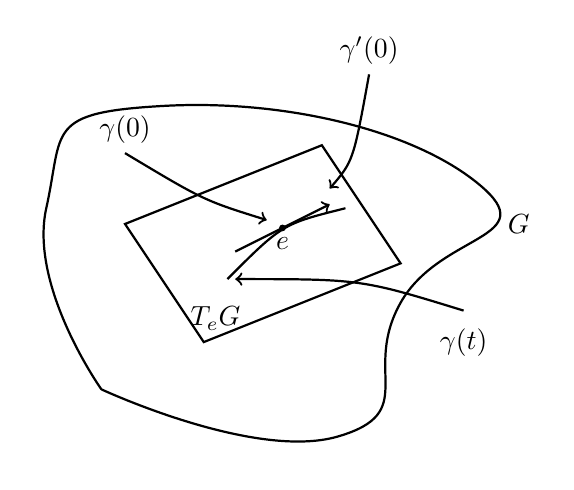
\begin{tikzpicture}
        
        % Draw the manifold G
        \draw[thick] plot [smooth,tension=1] 
        coordinates {(0.2,1.4) (3.2,0.8) (4,2.5) (5,4) (1,5) (-0.5,3.7) (0.2,1.4)};
        %\draw[thick] (0,0) to[out=30, in=180] (4,2.5) to[out=0, in=270] (5,4) to[out=90, in=30] (1,5) to[out=210, in=150] cycle;
        
        % Label G
        \node at (5.5,3.5) {$G$};
        
        % Draw the tangent space T_eG
        \draw[thick] (1.5, 2) -- (4, 3) -- (3, 4.5) -- (0.5, 3.5) -- cycle;
        
        % Label TeG
        \node at (1.65, 2.3) {$T_e G$};
        
        % Draw the curve \gamma(t)
        \draw[thick] (1.8, 2.8) .. controls (2.5, 3.5) .. (3.3, 3.7);
        
        % Label points and vectors
        \node at (0.5,4.7) {$\gamma(0)$};
        \draw[thick, ->] (0.5,4.4) .. controls (1.5,3.8) .. (2.3,3.55);
        \node at (4.8, 2) {$\gamma(t)$};
        \draw[thick, ->] (4.8,2.4) .. controls (3.5,2.8) .. (1.9,2.8);
        \filldraw[black] (2.5,3.45) circle (1pt) node[anchor=north] {$e$};
        \draw[thick, ->] (1.9, 3.15) -- (3.1, 3.75);
        \node at (3.6, 5.7) {$\gamma'(0)$};
        \draw[thick, ->] (3.6, 5.4) .. controls (3.4,4.3) .. (3.1,3.95);
        
    \end{tikzpicture}
\end{marginfigure}
由解的形式可见,对于$G$在幺元处的切空间$T_eG$的任意一个向量$A=\gamma'(0)$,就有$G$中的一元素$\gamma(1)=\exp(\gamma'(0))$与之对应.现在我们稍微总结一下:对于李群$G$这个流形,我们可以找到其单参数子群$T_eG$作为其切空间,并且我们可以找到一个指数映射从切空间到原空间,很快,当我们学会李代数的时候,我们会再次使用李代数的语言来总结:``李代数就是李群的切空间所导出的代数".

我们再次回到群$G$和它的单参数子群,我们发现,如果给定$G$中与幺元邻近的一个元素\sidenote[][]{当然,由于我们研究线性群,幺元为单位矩阵.}$g$,并定义向量$A=\log g$,则由$e^A=g$ 知,$A$ 为$G$ 在$e$ 处之切向量,$e^tA$为以 $A$ 为单位切向量的单参数子群.因此,对$G$ 中与幺元$e$ 邻近的一个元素就有$T_{e}(G)$($G$ 在幺元处的切空间)中一向量$A$ 与之对应,也就是说,设$U\subset G$ 中包含$e$ 的一个适当邻域,我们建立了一种对应关系
\begin{equation}
    \begin{aligned}
        G\supset U&\overunderset{\log}{\exp}{\longleftrightarrow}T_{e}(G)\\g&\to A=\log g\\e^{A}&\leftarrow A
    \end{aligned}
\end{equation}
这种对应关系可以使我们对李群的研究转化到与其对应的在幺元$e$处的切空间$T_e(G)$.而我们知道,$T_e(G)$是由向量组成的线性空间,其线性结构具有先天优势,拥有远比李群简单的结构和运算.但由于我们前面所提到的,由于矩阵乘法相比于数乘的不可交互性,自然由此导出的切空间的运算自然也不能简单用普通加减法来表述,即右侧关系图
\marginnote[]{$$\begin{aligned}&T_{e}(G)\qquad G\\&A\quad\longrightarrow\quad e^{A}\\&B\quad\longrightarrow\quad e^{B}\\&A+B\to e^{A+B}\ne e^{A}e^{B}\end{aligned}$$}

为此,我们迫切需要引入一种新的代数结构来反映$G$中的不可交换性,而具有这种新结构的线性空间$T_e(G)$
,就是我们下一节所要讲的\textbf{李代数}.
\section{李群与李代数}
\subsection{李代数}
由上面的讨论,我们现在知道$e^Ae^B\ne e^{A+B}$,那么,问题自然变为:$e^Ae^B=e^{?}$,或者表述为,$G$的单参数子群的代数结构是什么样的?

为了解决这个问题,我们设$A,B\in T_e(G)$,取一个参数$t$,并要求$|t|$适当小,从而能够保证$e^{tA}$与$e^{tB}$均为李群$G$中与幺元$e$邻近的元素\sidenote[][]{这个要求是必要的,我们需要满足后续使用级数的收敛性.}.现在我们构造一个函数:
\begin{equation}
    g(t)=e^{tA}e^{tB}e^{-tA}e^{-tB}
\end{equation}
显然,对于特例,即如果$e^{tA}$与$e^{tB}$可交换,$g(t)=e=\textbf{1}$,对于不可交换的情况,$g(t)$与幺元$e$的偏离程度反映了$e^{tA}$与$e^{tB}$的乘法与可交换的乘法之间的差异大小.现在我们具体分析$g(t)$.
\marginnote[*-2]{展开的计算过程
$$\begin{aligned}
    g(t)& =e^{tA}e^{tB}e^{-tA}e^{-tB} \\
    &=(\textbf{1}+tA+\frac{t^{2}}{2!}A^{2}+\frac{t^{3}}{3!}A^{3}+\cdots)(\textbf{1}+tB+\frac{t^{2}}{2!}B^{2}+\frac{t^{3}}{3!}B^{3}+\cdots) \\
    &(\textbf{1}-tA+\frac{t^2}{2!}A^2-\frac{t^3}{3!}A^3+\cdots)(\textbf{1}-tB+\frac{t^2}{2!}B^2-\frac{t^3}{3!}B^3+\cdots) \\
    &=\{\textbf{1}+t(A+B)+t^{2}(\frac{A^{2}}{2}+AB+\frac{B^{2}}{2})\\&+t^{3}(\frac{A^{3}}{6}+\frac{A^{2}B}{2}+\frac{AB^{2}}{2}+\frac{B^{3}}{6})+O(t^{4})\} \\
    &\{\textbf{1}-t(A+B)+t^2(\frac{A^2}{2}+AB+\frac{B^2}{2})\\&-t^3(\frac{A^3}{6}+\frac{A^2B}{2}+\frac{AB^2}{2}+\frac{B^3}{6})+O(t^4)\} \\
    &=\textbf{1}+t(A+B-A-B)+t^{2}(AB-BA)+t^{3}(\frac{A^{2}B}{2}-\frac{AB^{2}}{2} \\
    &-\frac{B^2A}{2}+\frac{BA^2}{2}-ABA+BAB)+O(t^4) \\
    &=\textbf{1}+t^{2}[A,B]+\frac{t^{3}}{2}([A,[A,B]]-[B,[B,A]])+O(t^{4})
\end{aligned}$$
}
\begin{equation}
    \begin{aligned}
        g(t)& =e^{tA}e^{tB}e^{-tA}e^{-tB} \\
        &=\textbf{1}+t^{2}[A,B]+\frac{t^{3}}{2}([A,[A,B]]-[B,[B,A]])+O(t^{4})
    \end{aligned}
\end{equation}
这里我们使用了对易子记号$[,]$,不过对于李代数,它也称为李括号,李乘法\sidenote[][*5]{事实上,对于线性群它等同于对易子,后面会加以区分的使用对易子和李括号.}.对于函数$g(t)$,我们有
\begin{equation}
    \frac{g(t)-\textbf{1}}{t^2}=[A,B]+O(t)
\end{equation}
因此,考虑极限$t\to0$时,
\begin{equation}
    \lim_{t\to0}\frac{g(t)-\textbf{1}}{t^{2}}=[A,B]
\end{equation}
由此,我们发现李群$G$的元素$e^{tA}$与$e^{tB}$的乘法的不可交换程度在$|t|$很小时主要取决于$[A,B]$

现在我们做变量代换$t=\sqrt{s}$,则
\begin{equation}
    \frac{g(\sqrt{s})-g(0)}{s}=[A,B]+O(\sqrt{s})
\end{equation}
并因此
\begin{equation}
    \lim_{s\to0}\frac{g(\sqrt{s})-g(0)}{s}=[A,B]
\end{equation}
这也说明$[A,B]$是李群$G$中过幺元的曲线$g(\sqrt{s})$在幺元处的\textbf{切向量},即$[A,B]\in T_e(G)$,这也意味着我们证明了如下关系
\begin{equation}
    \forall A,B\in T_{e}(G) , [A,B]\in T_{e}(G)
\end{equation}
即对易子(李括号)对向量空间$T_e(G)$的封闭性.


此时,我们可以回答开头所提到的问题了,不妨设$e^{tA}e^{tB}=e^{tC}$,则
\marginnote[]{展开的计算过程
$$\begin{aligned}
    tC&=\log e^{tC}=\log e^{tA}e^{tB}\\
    &=\log\{(\textbf{1}+t(A+B)+\frac{t^{2}}{2}(A^{2}+2AB+B^{2})+ \\
    &\quad+\frac{t^{3}}{6}(A^{3}+3A^{2}B+3AB^{2}+B^{3})+O(t^{4})\} \\
    &=t(A+B)+\frac{t^{2}}{2}(A^{2}+2AB+B^{2})+\frac{t^{3}}{6}(A^{3}+3A^{2}B+3AB^{2}+B^{3}) \\
    &\quad+O(t^{4})-\{t(A+B)+\frac{t^2}{2}(A^2+2AB+B^2)+O(t^3)\}^2/2+ \\
    &\quad+\{t(A+B)+\frac{t^{2}}{2}(A^{2}+2AB+B^{2})+O(t^{3})\}^{3}/3+O(t^{4}) \\
    &=t(A+B)+\frac{t^{2}}{2}(AB-BA)+\frac{t^{3}}{12}(A^{2}B-ABA-ABA+BA^{2} \\
    &\quad-B^2A+BAB+BAB-AB^2)+O(t^4) \\
    &=(tA+tB)+\frac{1}{2}[tA,tB]+\frac{1}{12}[tA,[tA,tB]-tB,[tB,tA]]+O(t^{4}) 
\end{aligned}$$}
\begin{equation}
\begin{aligned}
    tC&=\log e^{tC}=\log e^{tA}e^{tB}\\
    &=(tA+tB)+\frac{1}{2}[tA,tB]+\frac{1}{12}[tA,[tA,tB]-tB,[tB,tA]]+O(t^{4}) 
\end{aligned}
\end{equation}
由此可见,只要给出李括号,$T_e(G)$中知道了与$e^{tA},e^{tB}$相对应的元素$tA,tB$即可求得$T_e(G)$中与$e^{tA}e^{tB}$相对应的元素.因此,我们认为李括号可以表述李群切空间的代数结构,并对于李括号有如右侧所示的性质.
\marginnote[]{李括号的性质$$\begin{gathered}
        \left\lbrack {A, A}\right\rbrack = 0\\
        \left\lbrack {A, B}\right\rbrack = - \left\lbrack {B, A}\right\rbrack\\
        \left\lbrack {A, c}\right\rbrack = 0\;\left( {c\text{ 只是一个数 }}\right)\\
        \left\lbrack {A + B, C}\right\rbrack = \left\lbrack {A, C}\right\rbrack + \left\lbrack {B, C}\right\rbrack\\
        \left\lbrack {A,{BC}}\right\rbrack = \left\lbrack {A, B}\right\rbrack C + B\left\lbrack {A, C}\right\rbrack\\
        \left\lbrack {A,\left\lbrack {B, C}\right\rbrack }\right\rbrack + \left\lbrack {B,\left\lbrack {C, A}\right\rbrack }\right\rbrack + \left\lbrack {C,\left\lbrack {A, B}\right\rbrack }\right\rbrack = 0
    \end{gathered}$$}

我们称有了李括号的向量空间$T_e(G)$构成一个李代数,更准确的来讲是李群$G$的李代数,并记为$\mathfrak{g}$.\\
李群的李代数完全刻画了李群在幺元附近的结构,而要研究李群在幺元附近的性质只需要研究李代数即可,但是需要注意的是,李代数\textbf{仅}刻画了李群在幺元附近的\textbf{局部}性质,\textbf{不能}反映其整体性质,一个李群对应一个李代数,而一个李代数可以对应多个李群.
\begin{definition}[结构常数]
    设$G$是一个$r$维李群,取定幺元$e$的一个邻域$U$,在$U$中取定坐标系$\{U,\varphi\}$并取$e$为坐标原点:
    \begin{equation}
        \varphi(e)=(0,0,\cdots,0)
    \end{equation}
    对于其的单参数子群,我们有
    \begin{equation}
        \begin{cases}\gamma_j(t),&j=1,2,\cdots,r\\\varphi(\gamma_j(t))=(\underbrace{0,\cdots,0}_{(j-1)\text{个零}},t,0,\cdots,0)\end{cases}
    \end{equation}
    为其$r$条坐标曲线.
    
    以$X_{j}= \gamma _{j}^{\prime }(0),j= 1, 2, \cdots , r$记为其在幺元处的切向量.即$X_j\in T_e(G) = \mathfrak{g}, j= 1, 2, \cdots , r$.显然,$\{X_1,X_2,\cdots,X_r\}$可取作为向量空间$T_{_e}(G)$的基——$T_{e}(G)$中任一向量可用它们的线性组合表出.由于$[X_i,X_j]\in \mathfrak{g}$,所以
    \begin{equation}
        [X_{i},X_{j}]=\sum_{j,k=1}^{n}C_{ij}^{k}X_{k}\quad i,j=1,2,\cdots,r
    \end{equation}
    这$r^3$个数$\{C_{ij}^k\}k,i,j=1,2,\cdots,r$称为李群以$\{X_1,X_2,\cdots,X_r\}$,为基的\underline{结构常数}.
\end{definition}
对于李代数$\mathfrak{g}$中任意向量$X,Y$,有
\begin{equation}
    \begin{aligned}
        X&=\sum_{j=1}^{r}\xi^{j}X_{j}&Y=\sum_{j=1}^{r}\eta^{j}X_{j}\\
        X&\sim(\xi^{1},\xi^{2},\cdots,\xi^{r})&Y=(\eta^{1},\eta^{2},\cdots\eta^{r})\\
        Z&=[X,Y]=\left[\sum_{j=1}^{r}\xi^{j}X_{j},\sum_{k=1}^{r}\eta^{k}X_{k}\right]&=\sum_{i=1}^{r}\sum_{j,k=1}^{r}C_{jk}^{i_{k}}\xi^{j}\eta^{k}X_{i}
    \end{aligned}
\end{equation}
将$Z$也用坐标表示
\begin{equation}
    Z=\sum_{i=1}^{r}\zeta^{ i}X_{i},\quad Z\sim(\zeta^{ 1},\zeta^{ 2},\cdots\zeta^{ r})
\end{equation}
此时易求出结构常数
\begin{equation}
    \zeta^{i}=\sum_{j,k=1}^{r}C_{jk}^{i}\xi^{j}\eta^{k},\quad i=1,2,\cdots,r
\end{equation}
由此可见,结构常数可以完全确定一个李代数.

需要强调的是,结构常数与基的选取有关,而李代数的一个重要的问题就是如何选取适当的基使结构常数最简单.\\
或许到此,你可能还对结构常数一头雾水,在再次讲解结构常数之前,我们还是先给出一些基本性质,并实际算一下结构常数.
\begin{equation}
    \begin{aligned}
        &C_{ij}^{ k}=-C_{ji}^{ k}&i,j,k=1,2,\cdots,r\\
        &\sum_{l=1}^{r}\left(C_{ij}^{l}C_{lk}^{m}+C_{jk}^{l}C_{li}^{m}+C_{ki}^{l}C_{lj}^{m}\right)=0&i,j,k,m=1,2,\cdots,r.\end{aligned}
\end{equation}
\begin{example}
    我们再次考虑由例题3.8给出的群$T_2=\Big\{\begin{bmatrix}e^{x_1}&x_2\\0&1\end{bmatrix}\Big|x_1,x_2\in\mathbb{R}\Big\}$,我们知道$\gamma_1(t)=\begin{bmatrix}e^t&0\\0&1\end{bmatrix} -\infty<t<\infty $与$\gamma_2(t)=\begin{bmatrix}1&t\\0&1\end{bmatrix} -\infty<t<\infty $是$T_2$的两个单参数子群,同时也是过幺元的两条曲线,我们给出在幺元处的切向量$X_1=\gamma_1'(0)=\begin{bmatrix}1&0\\0&0\end{bmatrix},X_2=\gamma_2'(0)=\begin{bmatrix}0&1\\0&0\end{bmatrix}$,因此李群$T_2$的李代数$\mathfrak{t}_2$的基由$X_1,X_2$组成,现在来求结构常数.
    \begin{equation}
        \begin{aligned}&[X_1,X_1]=\begin{bmatrix}0&0\\0&0\end{bmatrix}\quad[X_2,X_2]=\begin{bmatrix}0&0\\0&0\end{bmatrix}\\&[X_1,X_2]=\begin{bmatrix}1&0\\0&0\end{bmatrix}\begin{bmatrix}0&1\\0&0\end{bmatrix}-\begin{bmatrix}0&1\\0&0\end{bmatrix}\begin{bmatrix}1&0\\0&0\end{bmatrix}=\begin{bmatrix}0&1\\0&0\end{bmatrix}=X_2.\end{aligned}
    \end{equation}
    所以,$C_{11}^1=C_{11}^2=C_{22}^1=C_{22}^2=0,\quad C_{12}^1=-C_{21}^1=0,\quad C_{12}^2=1,\quad C_{21}^2=-1.$
\end{example}
\begin{example}
    我们再次回到$SO(3)$群,现在我们来求其李代数$\mathfrak{so}(3)$及其结构常数.\\
    我们列出其群元(绕$x,y,z$的转动),即旋转矩阵,如右侧所示
        \marginnote[*-3]{三个群元的矩阵表示:
        $$g_{x}(t)=\begin{bmatrix}1&0&0\\0&\cos t&-\sin t\\0&\sin t&\cos t\end{bmatrix}$$
        $$g_y(t)=\begin{bmatrix}\cos t&0&\sin t\\0&1&0\\-\sin t&0&\cos t\end{bmatrix}$$
        $$g_{z}(t)=\begin{bmatrix}\cos t&-\sin t&0\\\sin t&\cos t&0\\0&0&1\end{bmatrix}$$
    }

    此时,我们发现,这是其的三个单参数子群,而它们在幺元处的切向量一并给出
    \begin{equation}
        I_{1}=g_{x}'(0),\quad I_{2}=g_{y}'(0),\quad I_{3}=g_{z}'(0).
    \end{equation}
    于是$\{I_1,I_2,I_3\}$构成$SO(3)$的李代数$\mathfrak{so}(3)$的一组基,其李括号为:
    \begin{equation}
        [I_1,I_2]=I_1I_2-I_2I_1=I_3,[I_2,I_3]=I_1,[I_3,I_1]=I_2
    \end{equation}
    同时得出结构常数$C_{12}^{ 1}=0,C_{12}^{ 2}=0,C_{12}^{ 3}=1,\cdots.$
    
    我们可以发现,对于这个李括号,其还等价于三维欧式空间的向量乘法,我们就得到了简单情况下的李括号的退化情况.
\end{example}

%\begin{example}
%	我们这次要讨论的是在物理上极为重要的一类李群:$SU(2)$
%\end{example}
\subsection{李氏三定理和无穷小变换}
1
\subsection{李群的无穷小生成元}
1
\subsection{典型李群和李代数}
1
\section{李代数进阶}
\subsection{张量,不可约张量}
1
\subsection{卡西米尔算符(Casimir operator)}
1
\subsection{典型李代数的二阶卡西米尔算符}
1


